\chapter{Interfaz}
\label{cap:interfaz}

En cuanto a la interfaz de la página web, uno de los principales objetivos del presente trabajo era aunar todas las funcionalidades de la aplicación original, así como las extensiones implementadas en este desarrollo, en una única interfaz web, mediante la cual el usuario pueda navegar y acceder a todas las funcionalidades disponibles.

El resultado de este objetivo está recogido en este capítulo. Para alcanzarlo, se han creado vistas completamente nuevas y se han modificado algunas de las vistas previamente existentes para simplificarlas o añadir funcionalidades.

Atendiendo a la movilidad entre páginas, se ha implementado una barra de navegación, la cual compartirán todas las páginas y permitirá navegar entre las diferentes funcionalidades, como se puede apreciar en las figuras \ref{fig:navBarDesktop} y \ref{fig:navBarMobile}.

\begin{figure}[h]
	\centering
	
\includegraphics[width = 1\textwidth]{Imagenes/Vectorial/navBarDesktop.png}
	\caption{Barra de navegación en el formato Desktop}
	\label{fig:navBarDesktop}
\end{figure}

\begin{figure}[h]
	\centering
	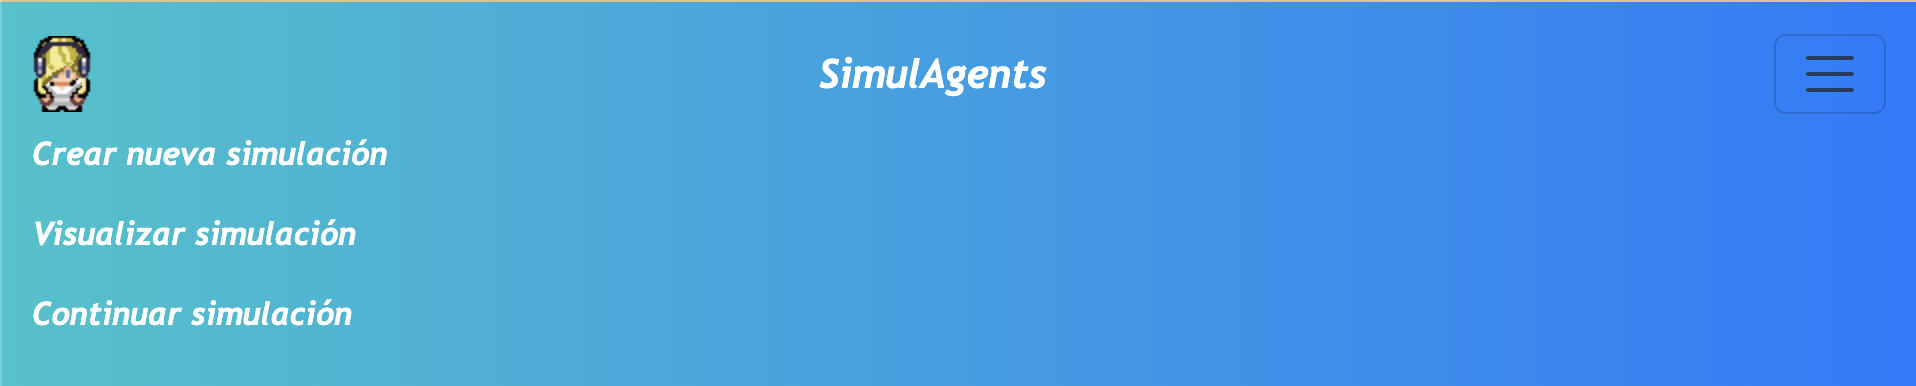
\includegraphics[width = 1\textwidth]{Imagenes/Vectorial/navBarMobile.png}
	\caption{Barra de navegación en el formato para dispositivos móviles}
	\label{fig:navBarMobile}
\end{figure}

\section{Nuevas vistas}

En esta sección se presentan las vistas creadas durante el desarrollo del trabajo, las cuales sirven de apoyo para ejecutar las funcionalidades, tanto nuevas como existentes, de la aplicación.

\subsection{Vista de Crear nueva simulación}

Teniendo en cuenta los objetivos y las funcionalidades implementadas en este trabajo, es evidente la necesidad de un apartado en el que permitir a los usuarios crear sus propias simulaciones. En esta vista, los usuarios primeramente indicarán el número de personajes que quieren que intervengan en la simulación.

Dependiendo del número de personajes deseados, mediante el uso de la tecnología JQuery, se mostrarán u ocultarán las casillas de relleno de la información de los personajes. Para cada uno de los agentes, los usuarios indicarán el nombre que le quieren dar y la personalidad de los mismos. En el apartado de personalidad ,se indican todas sus relaciones sociales preexistentes en lenguaje natural, así como los pensamientos y pretensiones que el agente tiene al inicio de la simulación.

Por último, hay un apartado de contexto de la simulación, en el cual los usuarión deberán insertar todo el contexto de la situación en la que se ejecute la simulación. En esta información entraría el día en el que se ejecuta, la situación en la que se encuentran los personajes y todo tipo de información que pueda aportar contexto a la simulación.

Todas estos elementos gráficos se pueden apreciar en la figura \ref{fig:vistaCrearSimulacion}.

\begin{figure}[h]
	\centering
	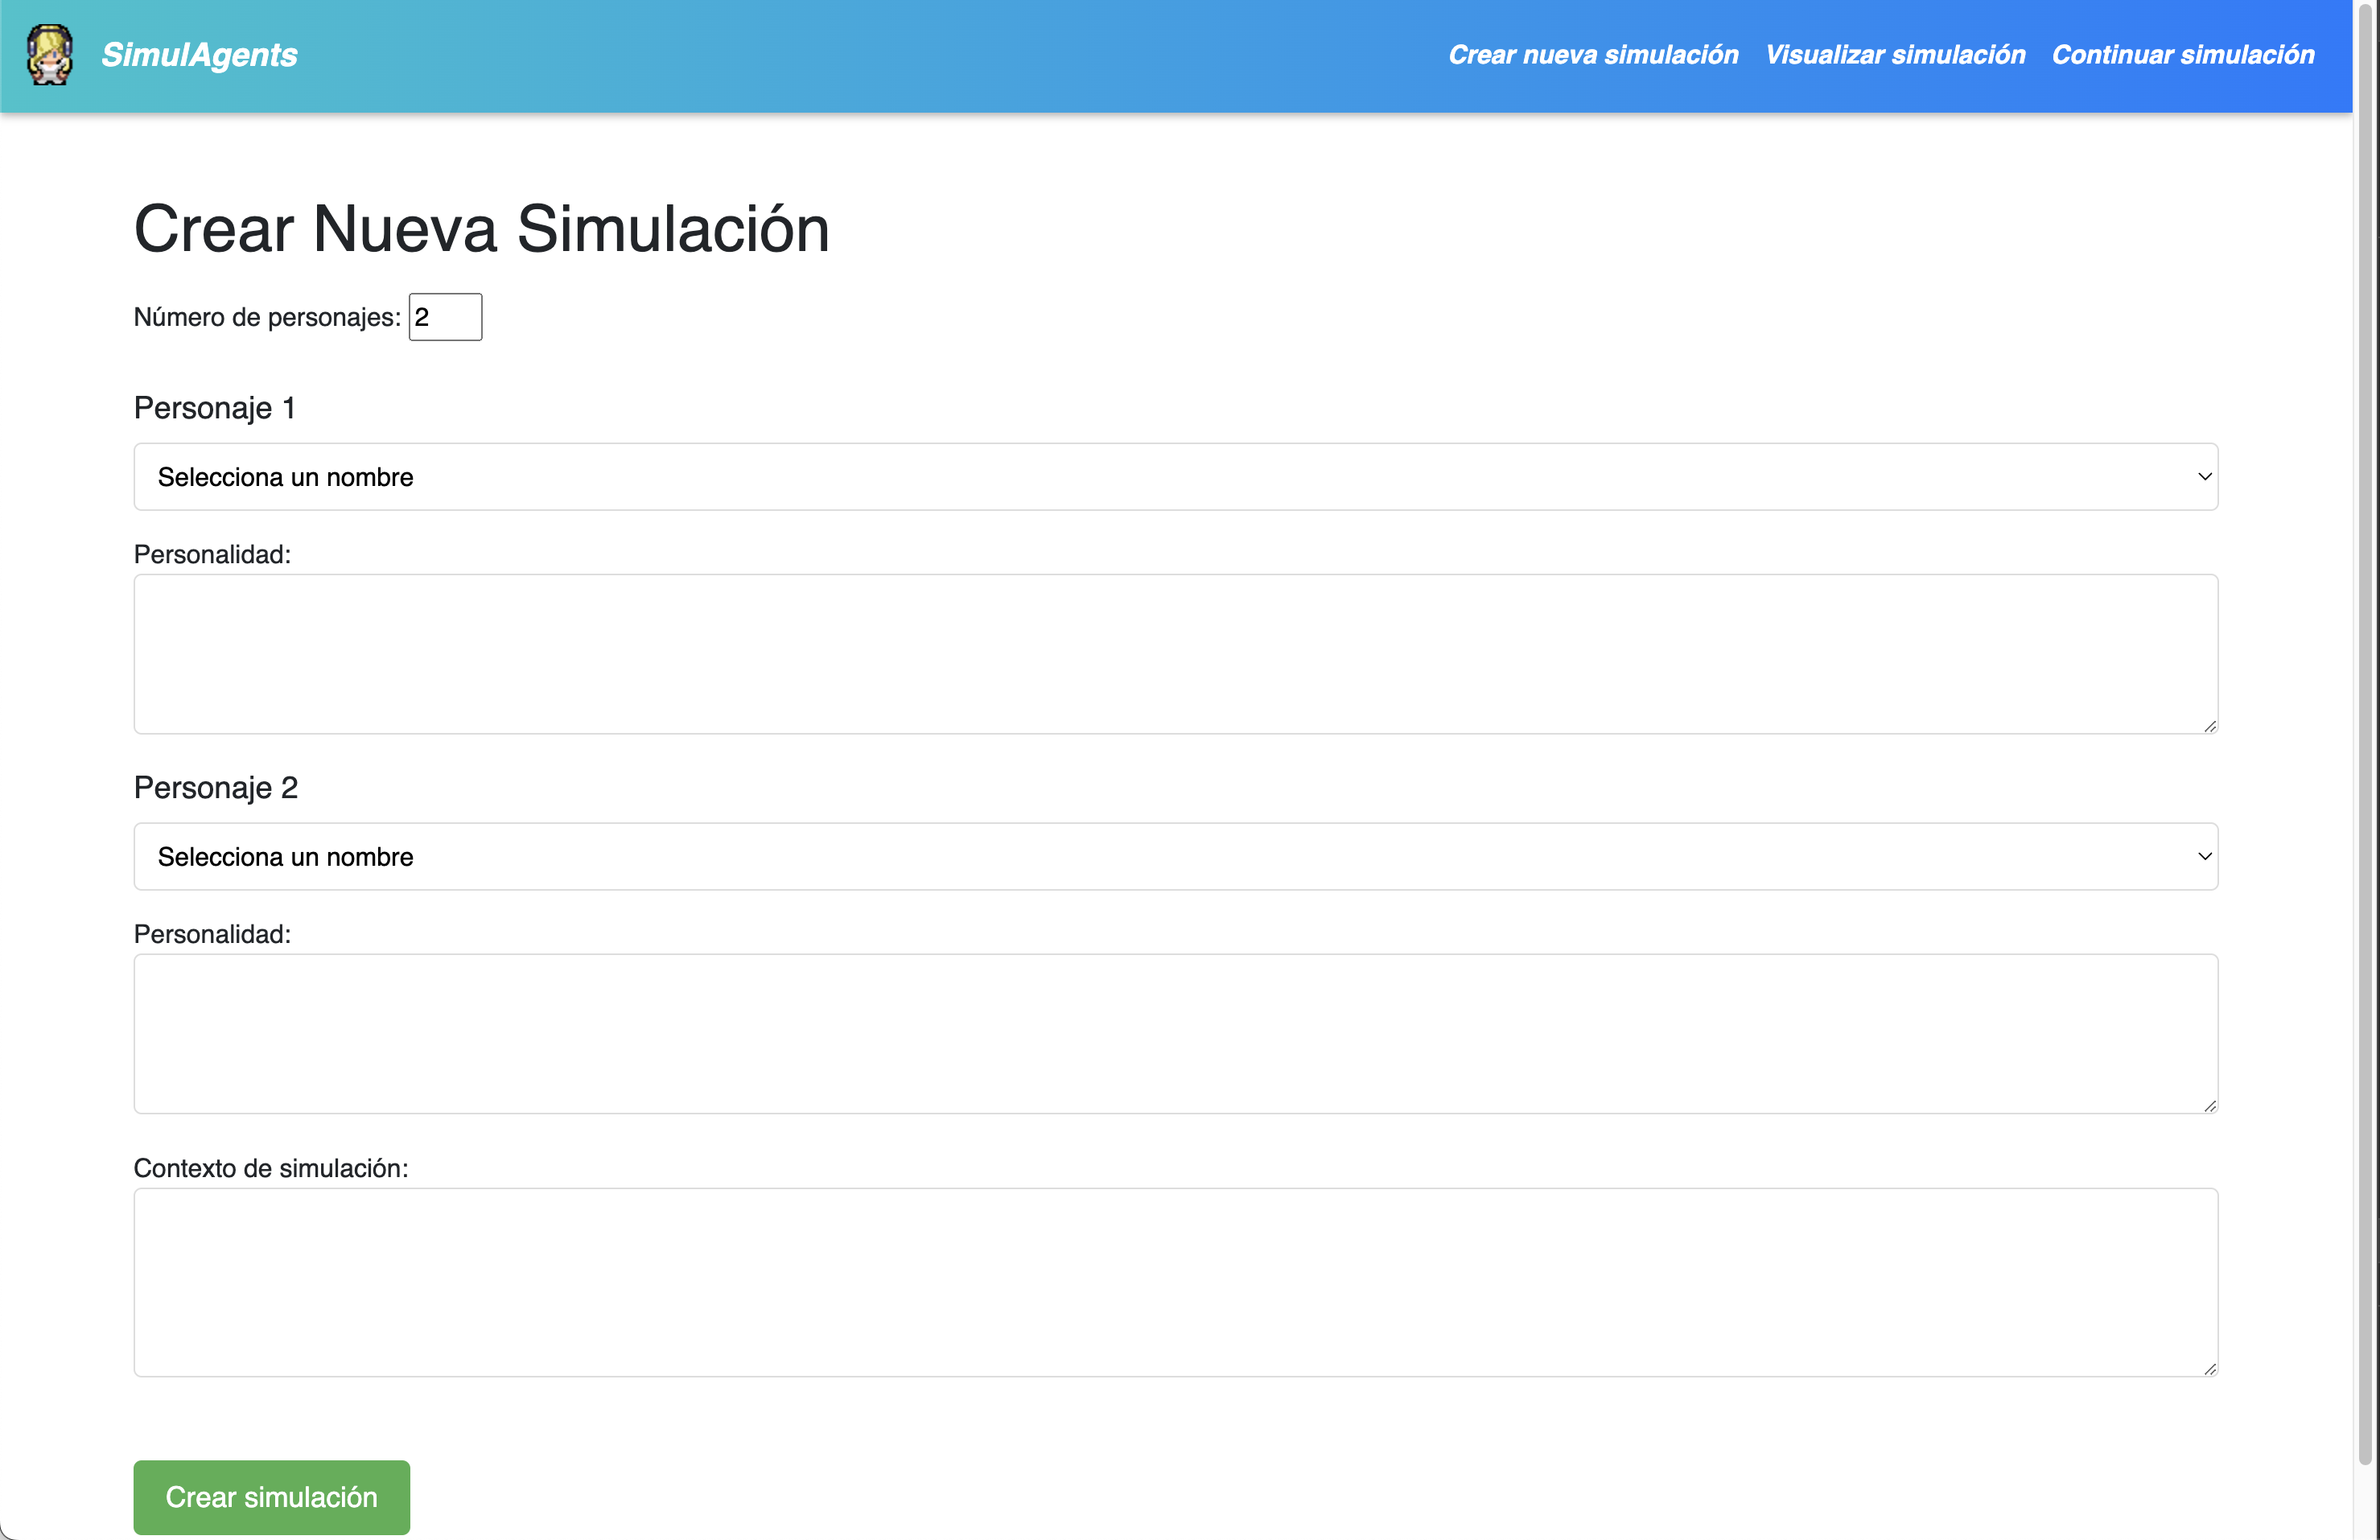
\includegraphics[width = 1\textwidth]{Imagenes/Vectorial/vistaCrearSimulacion.png}
	\caption{Versión de escritorio de la vista para crear una nueva simulación}
	\label{fig:vistaCrearSimulacion}
\end{figure}

\textcolor{red}{CAMBIAR ESTA FOTO POR LA VISTA FINAL REAL}

\subsection{Vista de Visualizar simulación}

En esta vista es donde los usuarios pueden seleccionar las simulaciones a visualizar. Esto es, las que se han ejecutado y guardado para visualizarlas previamente.

En cada simulación se puede apreciar cierta información importante sobre la misma, como puede ser el título de la simulación, un link que redirige a la simulación original desde la que ha sido guardada, un resumen de la misma, indicando el mapa en a en el que se ha realizado, los mejores momentos con los steps exactos, \textcolor{red}{PONER LO QUE HABRÁ EN CADA SIMULACIÓN}

Como ejemplo, se proporcionan las figuras (\textcolor{red}{PONER LAS FIGURAS}) para ver cómo aparece esta vista representada en la página web.


\subsection{Vista de Continuar simulación}

La vista de continuar simulación es ciertamente similar a la anterior de visualizar simulación, ya que también habrá una lista con simulaciones, y alguna información sobre ellas, en este caso, cada simulación contendrá datos como el título de esta, \textcolor{red}{PONER LO QUE HABRÁ EN CADA SIMULACIÓN}

 En las figuras (\textcolor{red}{PONER LAS FIGURAS}) se puede apreciar el resultado de esta vista

\subsection{Vista de Guía de Usuario}

Además de las vistas creadas para navegar e interactuar con las simulaciones, se ha creado una página que sirve como guía de usuario. 

Como el uso de esta herramienta lo hemos orientado a perfiles no técnicos (como psicólogos o personas que quieran estudiar las interacciones sociales), se ha añadido esta sección en la que se explican todas las funcionalidades de la aplicación, cómo utilizarlas y algunos trucos o consejos de uso, para maximizar el valor del programa.

Algunos ejemplos de esta página son los que se muestran en las figuras (\textcolor{red}{PONER LAS FIGURAS})

\section{Vistas modificadas}

Además de las vistas creadas desde cero, había algunas que ya estaban creadas (como las de la visualización o ejecución de la simulación, que requerían de un motor de videojuego corriendo). Sin embargo, para añadir ciertas funcionalidades, también se han modificado algunas de estas, las cuales se indican en la presente sección.

\subsection{Vista de landing}

Originalmente, cuando el usuario arrancaba el servidor, existía una página de landing a la que se le redirigía, donde se indicaba que el servidor se encontraba en funcionamiento. Como esta página era muy rudimentaria y tan solo contenía una línea de información, se decidió rediseñar la landing completamente, indicando las principales funcionalidades de la aplicación desde una interfaz intuitiva, sencilla y accesible.

El resultado de cómo se ve la vista de landing actualmente se puede ver en la figura \ref{fig:landing}

\begin{figure}[h]
	\centering
	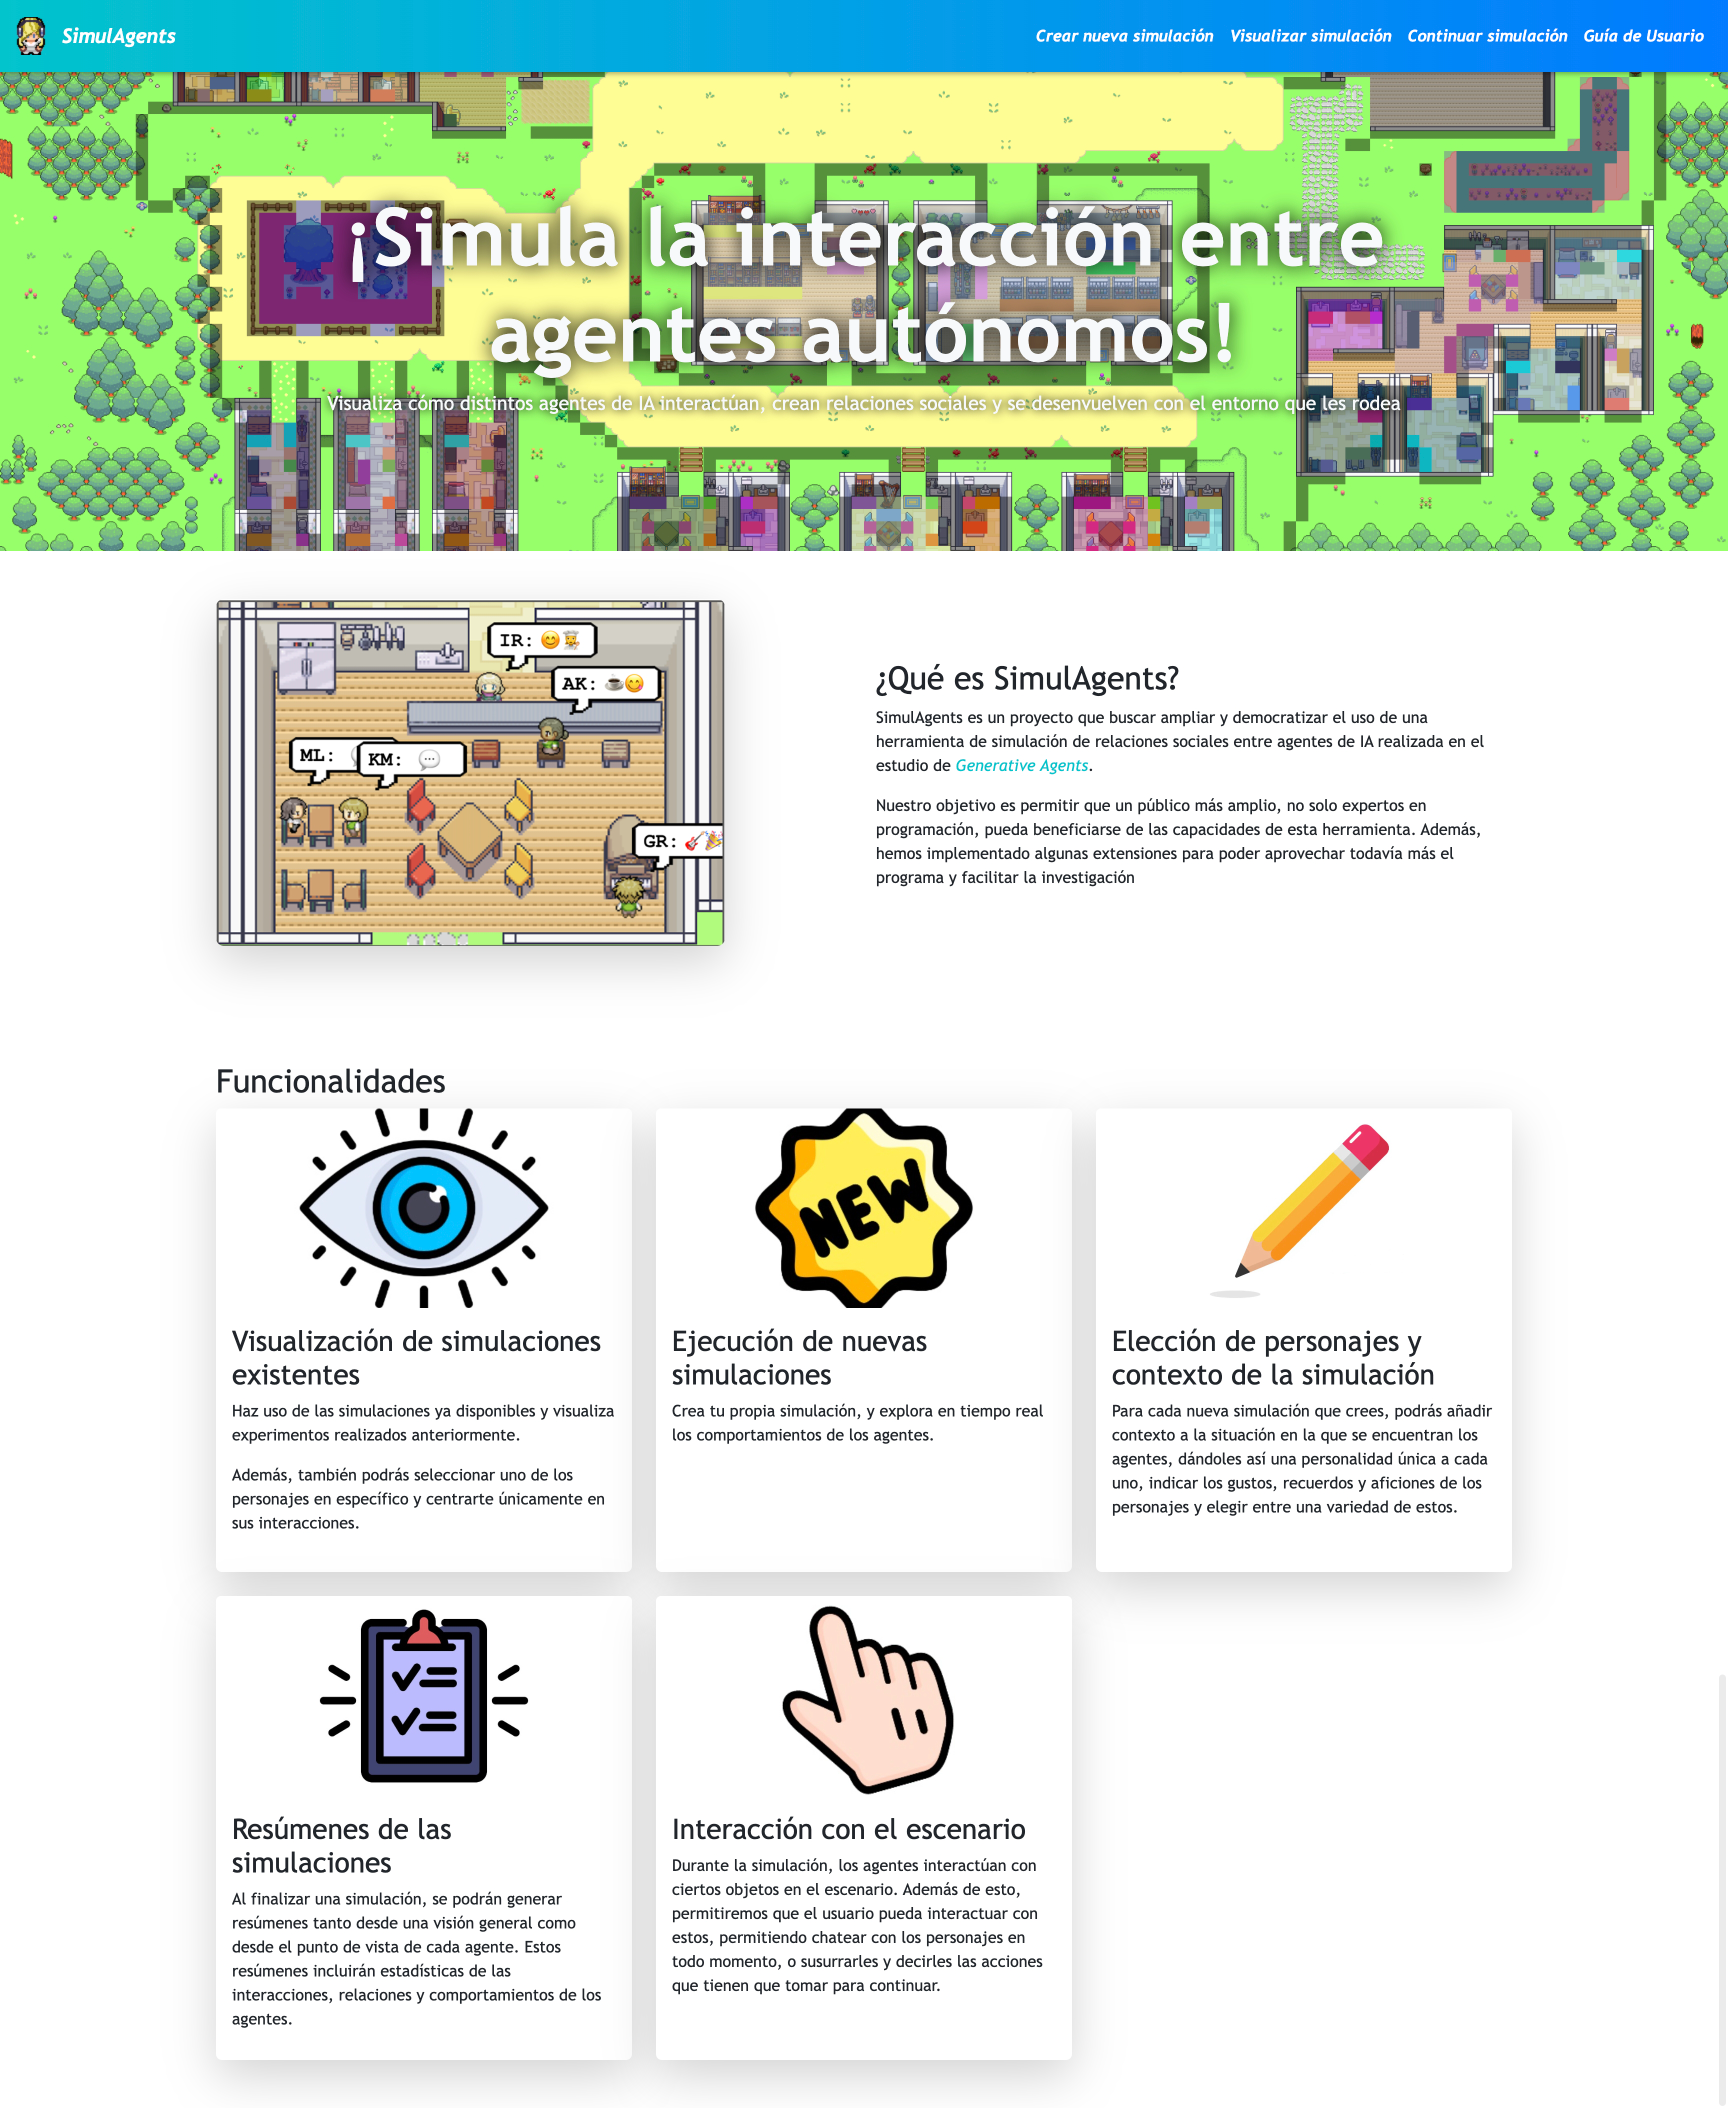
\includegraphics[width = 0.8\textwidth]{Imagenes/Vectorial/landing.png}
	\caption{Vista de landing actualizada}
	\label{fig:landing}
\end{figure}

\subsection{Botones de play y stop al ejecutar simulación}

\subsection{Botones de chat y susurro en la vista del personaje}
